\documentclass[11pt]{scrartcl}

\usepackage{ucs}
\usepackage[utf8]{inputenc}
\usepackage[T1]{fontenc}
\usepackage[ngerman]{babel}
\usepackage{amsmath,amssymb,amstext}
\usepackage{graphicx}
\usepackage{parskip}
\usepackage{hyperref}
\usepackage{float}
\usepackage{subfiles}
\usepackage{titling}
\usepackage{ccicons}
\usepackage{fontawesome}
\usepackage{subfig}
\usepackage[top=1in, bottom=1.25in, left=1.25in, right=1.25in]{geometry}
\usepackage{xcolor}
\usepackage{listings}
\usepackage{natbib}
\usepackage{enumerate}
\usepackage{longtable}
\usepackage[ddmmyyyy]{datetime}
\usepackage{pdfpages}
\usepackage{wrapfig}
\usepackage{pdflscape}
\renewcommand{\dateseparator}{.}

\lstset{basicstyle=\small,
    showstringspaces=false,
    commentstyle=\color{black},
    keywordstyle=\color{blue}
}

\bibliographystyle{unsrtnat}
\graphicspath{{images/},{images/Redlichkeitserklaerung/}}


    %\title{Dokumentation - PREN}
    \title{Schlussdokumentation PREN2 Gruppe 28}
    \author{Andreas Rebsamen (Elektrotechnik) \\Joel Grepper (Informatik)\\ Manuel Omlin (Maschinentechnik)\\ Marco Schöni (Maschinentechnik)\\ Patrick Marty (Informatik)\\ Steve Ineichen (Informatik)}
    \date{\today{}}

\begin{document}

    \begin{titlingpage}
        \begin{flushleft}
            \begin{Huge} %Exakter Modulnamen und Modulnamen ausgeschrieben
                %TA.BA{\_}PREN1.H1801 \\
                \textbf{\thetitle} \\
            \end{Huge}
            \vspace{1.5cm}
            \begin{large} %Author-Variable
                \theauthor \\
            \end{large}
            \vspace{1.5cm}
            \begin{huge}
                \textbf{Hochgeschwindigkeitsschienenfahrzeug}\\
                \textbf{''SOUL TRAIN''}\\
            \end{huge}
            \vspace{0.5cm}
            \begin{large}
                Hochschule Luzern – Technik \& Architektur\\
                TA.BA{\_}PREN2.F1901
            \end{large}
            \vspace{1.5cm}
            \begin{figure}[H] %Titelbild
                \centering
                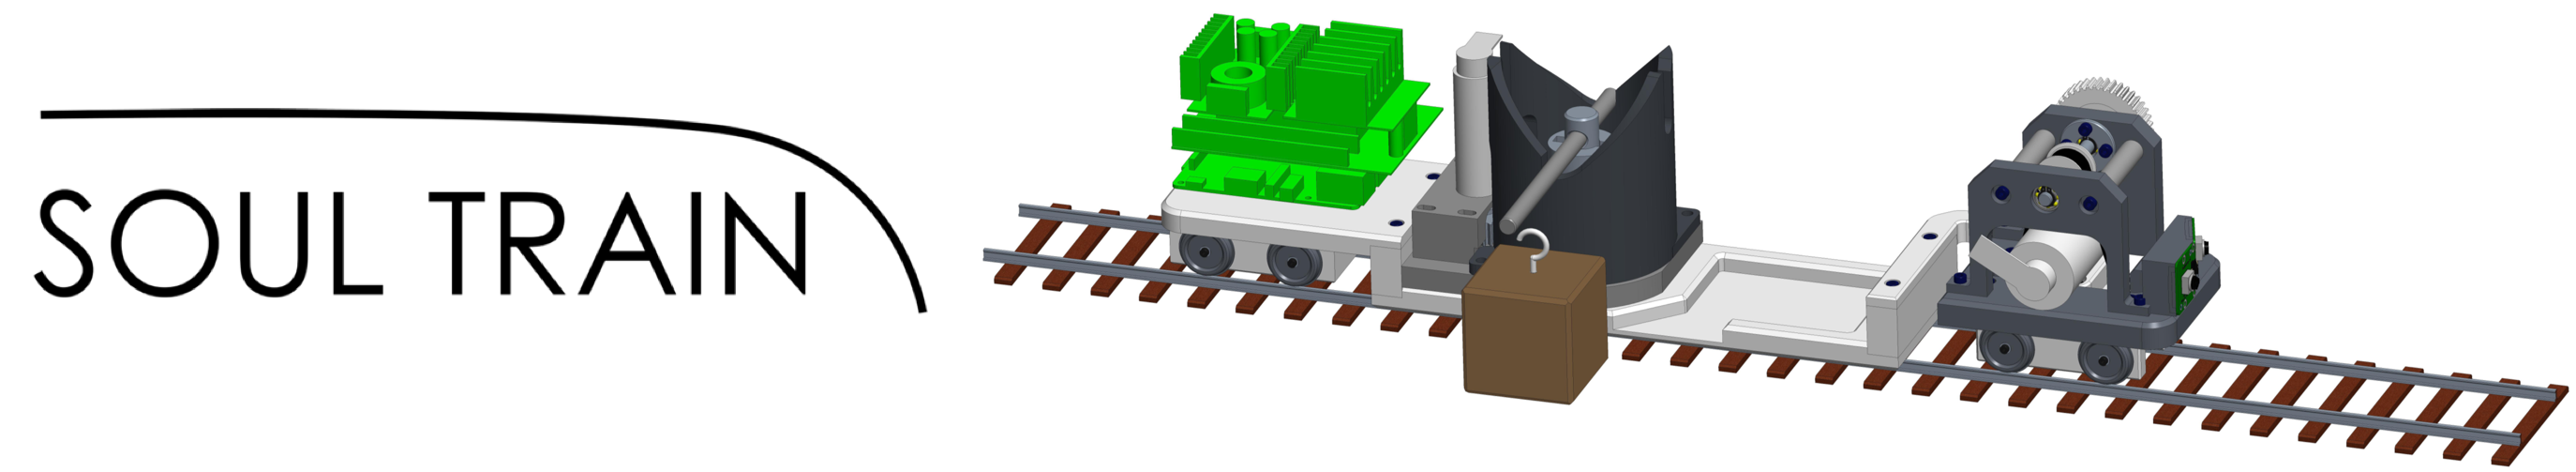
\includegraphics[width=1\textwidth]{images/soultrain.png}
            \end{figure}
            \vspace{3cm}
            \begin{large} %Datumsvariable
                Horw, Hochschule Luzern – Technik \& Architektur, \thedate
            \end{large}
        \end{flushleft}
    \end{titlingpage}

    %Redlichkeitserklärung
    \subfile{Redlichkeitserklaerung.tex}

    %Inhaltsverzeichnis
    \setcounter{tocdepth}{2}
    \tableofcontents
    \clearpage

    \section{Management Summary}
    \subfile{sections/01_ManagementSummery/managementSummery.tex}
    \clearpage

    \section{Einleitung}
    \subfile{sections/02_Einleitung/einleitung.tex}
    \clearpage

    \section{Produktbeschrieb}
    \subfile{sections/03_Produktbeschrieb/uebersicht.tex}
    \clearpage
    \subfile{sections/03_Produktbeschrieb/Wuerfelaufnahme.tex}
    \clearpage
    \subfile{sections/03_Produktbeschrieb/Fahrwerk.tex}
    \clearpage
    \subfile{sections/03_Produktbeschrieb/et_hw.tex}
    \clearpage
    \subfile{sections/03_Produktbeschrieb/et_sw.tex}
    \clearpage
    \subfile{sections/03_Produktbeschrieb/pi_tiny.tex}
    \clearpage
    % TODO: Kompiliert nicht mit diesem!
    \begin{Huge}
        \textbf{\color{red}{TODO: steuerungssoftware.tex einbinden}}
    \end{Huge}
    %\subfile{sections/03_Produktbeschrieb/steuerungssoftware.tex}
    \clearpage
    \subfile{sections/03_Produktbeschrieb/beschleunigungssensor.tex}
    \clearpage
    \subfile{sections/03_Produktbeschrieb/akustik.tex}
    \clearpage
    \subfile{sections/03_Produktbeschrieb/webApp.tex}
    \clearpage
    \subfile{sections/03_Produktbeschrieb/numberdetection.tex}
    \clearpage
 
    \section{Bewertung} \label{main_bewertung}
    \subfile{sections/04_Bewertung/bewertung.tex}
    \clearpage

    \section{Bedienungsanleitung}
    \subfile{sections/05_Bedienungsanleitung/Bedienungsanleitung_MT.tex}
    \subfile{sections/05_Bedienungsanleitung/bedienungsanleitung.tex}
    \clearpage

    \section{Schlussdiskusion}
    \subfile{sections/06_Schlussdiskussion/schlussdiskusion.tex}
    
    \clearpage
    \section{Verzeichnisse}
    \listoffigures
    \clearpage
    \listoftables
    \clearpage
    \bibliography{diverses/literatur-lib}
    \clearpage
\end{document}
